\documentclass{standalone}
\usepackage{tikz}
\usetikzlibrary{patterns, positioning}
\usepackage[sfdefault]{ClearSans} %% option 'sfdefault' activates Clear Sans as the default text font
\usepackage[T1]{fontenc}

\begin{document}
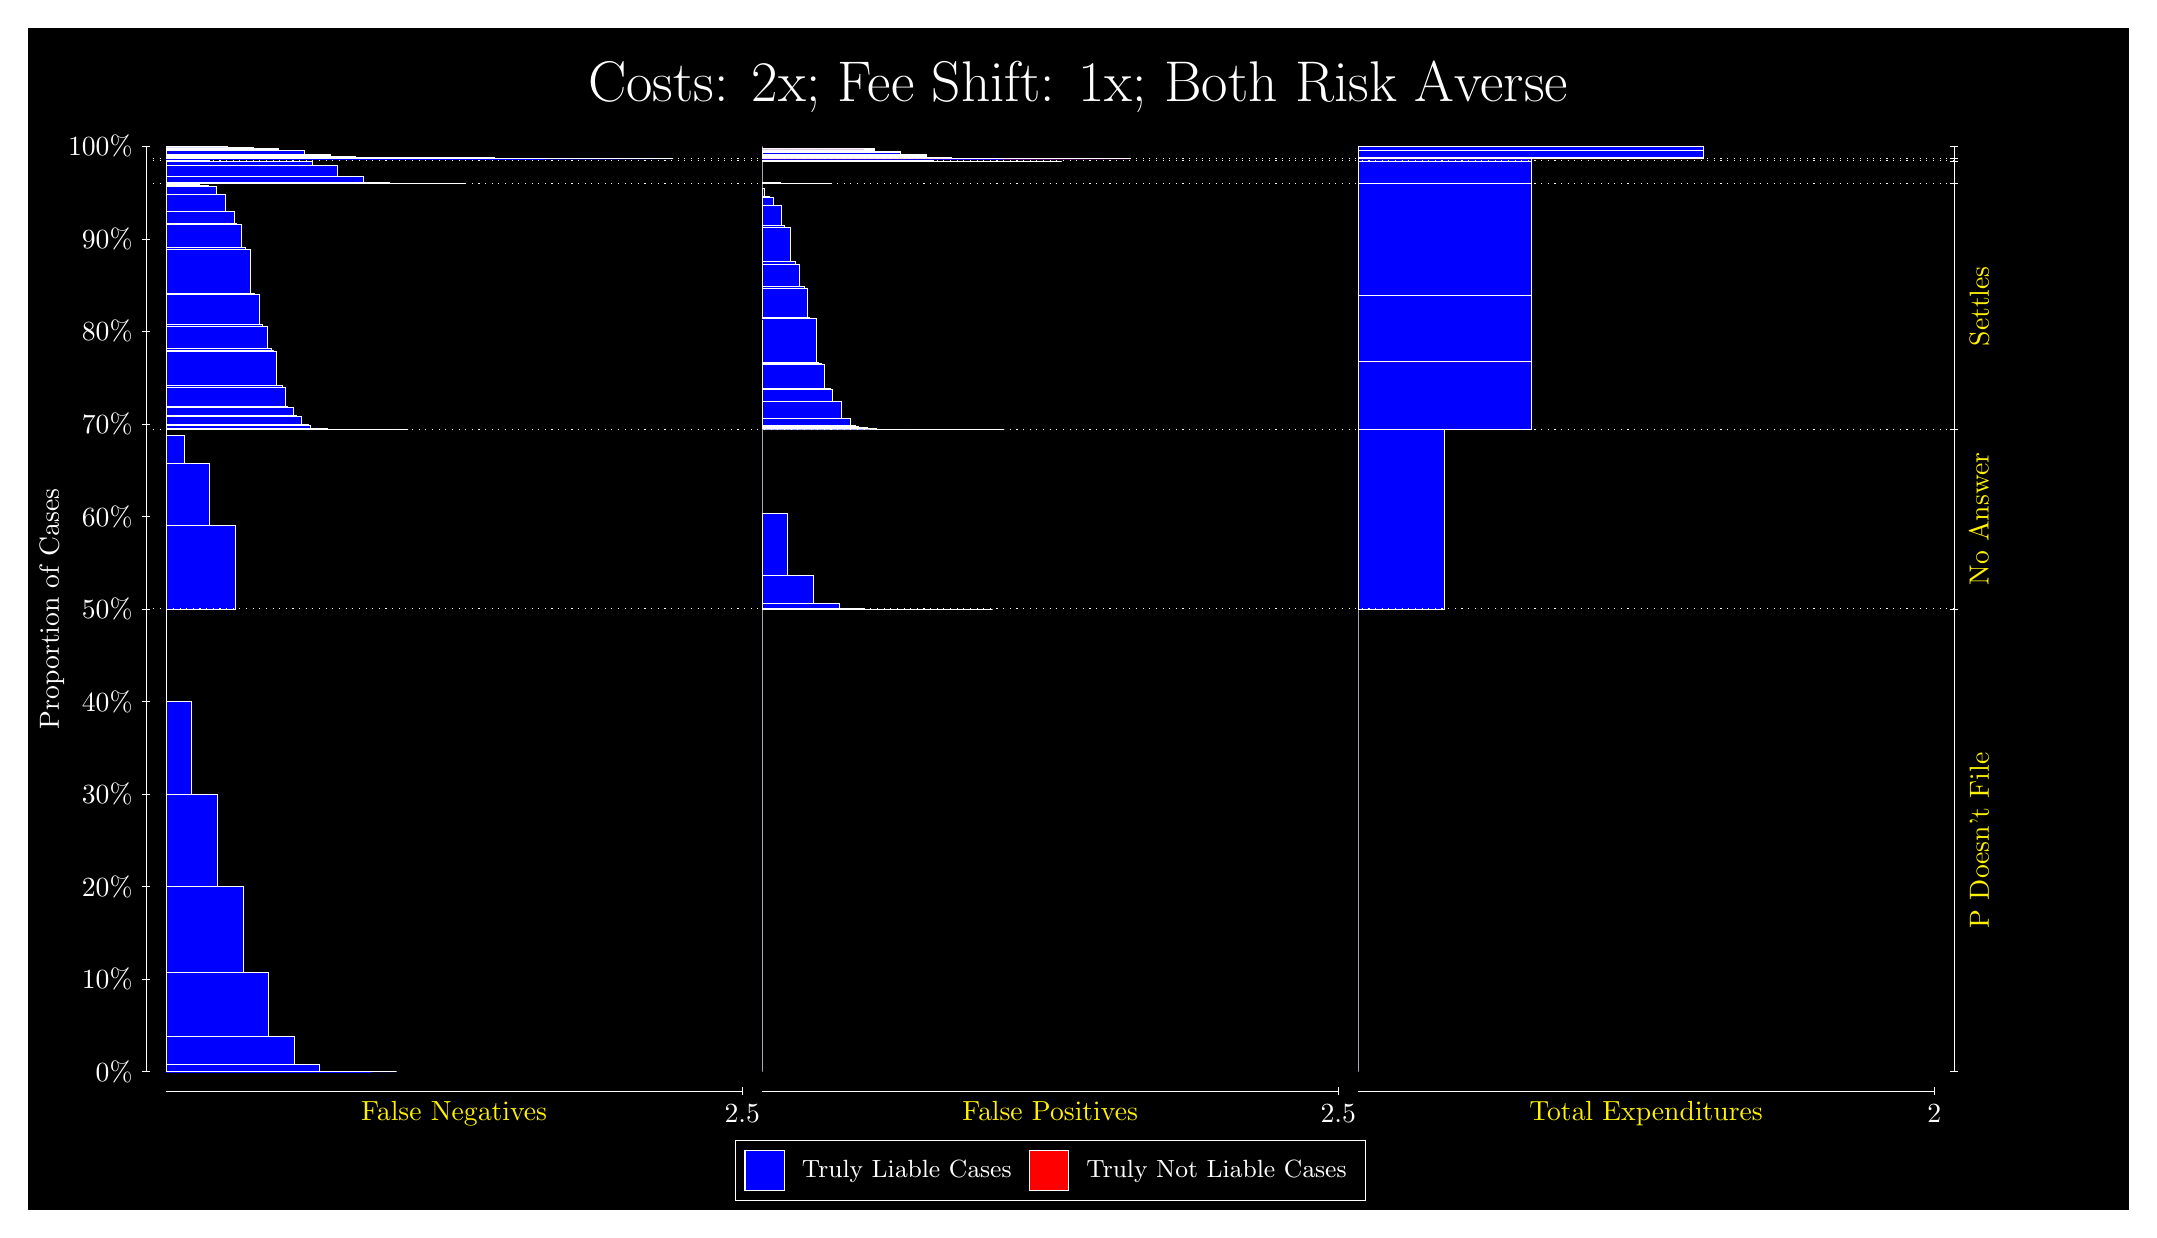
\begin{tikzpicture}
\draw[fill=black] (0,0) rectangle (26.667,15);
\draw[text=white] (0,13.5) rectangle (26.667,15) node[midway] {\huge Costs: 2x; Fee Shift: 1x; Both Risk Averse};
\draw[white, very thin] (1.5,1.75) -- (1.5,13.5);
\node[rotate=90, text=white, anchor=center] at (0.3, 7.625) {Proportion of Cases};
\draw[white, very thin] (1.45,1.75) -- (1.55,1.75);
\node[text=white, anchor=east] at (1.45, 1.75) {0\%};
\draw[white, very thin] (1.45,2.925) -- (1.55,2.925);
\node[text=white, anchor=east] at (1.45, 2.925) {10\%};
\draw[white, very thin] (1.45,4.1) -- (1.55,4.1);
\node[text=white, anchor=east] at (1.45, 4.1) {20\%};
\draw[white, very thin] (1.45,5.275) -- (1.55,5.275);
\node[text=white, anchor=east] at (1.45, 5.275) {30\%};
\draw[white, very thin] (1.45,6.45) -- (1.55,6.45);
\node[text=white, anchor=east] at (1.45, 6.45) {40\%};
\draw[white, very thin] (1.45,7.625) -- (1.55,7.625);
\node[text=white, anchor=east] at (1.45, 7.625) {50\%};
\draw[white, very thin] (1.45,8.8) -- (1.55,8.8);
\node[text=white, anchor=east] at (1.45, 8.8) {60\%};
\draw[white, very thin] (1.45,9.975) -- (1.55,9.975);
\node[text=white, anchor=east] at (1.45, 9.975) {70\%};
\draw[white, very thin] (1.45,11.15) -- (1.55,11.15);
\node[text=white, anchor=east] at (1.45, 11.15) {80\%};
\draw[white, very thin] (1.45,12.325) -- (1.55,12.325);
\node[text=white, anchor=east] at (1.45, 12.325) {90\%};
\draw[white, very thin] (1.45,13.5) -- (1.55,13.5);
\node[text=white, anchor=east] at (1.45, 13.5) {100\%};

\draw[white, very thin] (24.457,1.75) -- (24.457,13.5);
\draw[white, very thin] (24.407,1.75) -- (24.507,1.75);
\node[anchor=west] at (24.407, 1.75) {};
\draw[white, very thin] (24.407,7.625) -- (24.507,7.625);
\node[anchor=west] at (24.407, 7.625) {};
\draw[white, very thin] (24.407,9.9062) -- (24.507,9.9062);
\node[anchor=west] at (24.407, 9.9062) {};
\draw[white, very thin] (24.407,13.033) -- (24.507,13.033);
\node[anchor=west] at (24.407, 13.033) {};
\draw[white, very thin] (24.407,13.316) -- (24.507,13.316);
\node[anchor=west] at (24.407, 13.316) {};
\draw[white, very thin] (24.407,13.344) -- (24.507,13.344);
\node[anchor=west] at (24.407, 13.344) {};
\draw[white, very thin] (24.407,13.5) -- (24.507,13.5);
\node[anchor=west] at (24.407, 13.5) {};

\draw[white, very thin, fill=blue] (1.75,1.75) rectangle (4.6775,1.75);
\draw[white, very thin, fill=blue] (1.75,1.75) rectangle (4.3523,1.7503);
\draw[white, very thin, fill=blue] (1.75,1.7503) rectangle (4.027,1.7576);
\draw[white, very thin, fill=blue] (1.75,1.7576) rectangle (3.7017,1.8362);
\draw[white, very thin, fill=blue] (1.75,1.8362) rectangle (3.3764,2.1987);
\draw[white, very thin, fill=blue] (1.75,2.1987) rectangle (3.0511,3.0112);
\draw[white, very thin, fill=blue] (1.75,3.0112) rectangle (2.7258,4.1076);
\draw[white, very thin, fill=blue] (1.75,4.1076) rectangle (2.4006,5.2753);
\draw[white, very thin, fill=blue] (1.75,5.2753) rectangle (2.0753,6.45);
\draw[white, very thin, fill=red] (1.75,6.45) rectangle (1.75,6.45);
\draw[white, very thin, fill=blue] (1.75,6.45) rectangle (1.75,7.625);
\draw[white, very thin, fill=blue] (1.75,7.625) rectangle (2.6283,8.6865);
\draw[white, very thin, fill=blue] (1.75,8.6865) rectangle (2.303,9.4728);
\draw[white, very thin, fill=blue] (1.75,9.4728) rectangle (1.9777,9.828);
\draw[white, very thin, fill=red] (1.75,9.828) rectangle (1.75,9.828);
\draw[white, very thin, fill=blue] (1.75,9.828) rectangle (1.75,9.9062);
\draw[white, very thin, fill=blue] (1.75,9.9062) rectangle (4.8239,9.9062);
\draw[white, very thin, fill=blue] (1.75,9.9062) rectangle (4.6775,9.9062);
\draw[white, very thin, fill=blue] (1.75,9.9062) rectangle (4.5312,9.9062);
\draw[white, very thin, fill=blue] (1.75,9.9062) rectangle (4.4986,9.9062);
\draw[white, very thin, fill=blue] (1.75,9.9062) rectangle (4.3848,9.9062);
\draw[white, very thin, fill=blue] (1.75,9.9062) rectangle (4.3523,9.9062);
\draw[white, very thin, fill=blue] (1.75,9.9062) rectangle (4.2384,9.9062);
\draw[white, very thin, fill=blue] (1.75,9.9062) rectangle (4.2059,9.9062);
\draw[white, very thin, fill=blue] (1.75,9.9062) rectangle (4.1734,9.9062);
\draw[white, very thin, fill=blue] (1.75,9.9062) rectangle (4.092,9.9062);
\draw[white, very thin, fill=blue] (1.75,9.9062) rectangle (4.0595,9.9062);
\draw[white, very thin, fill=blue] (1.75,9.9062) rectangle (4.027,9.9062);
\draw[white, very thin, fill=blue] (1.75,9.9062) rectangle (3.9457,9.9062);
\draw[white, very thin, fill=blue] (1.75,9.9062) rectangle (3.9131,9.9083);
\draw[white, very thin, fill=blue] (1.75,9.9083) rectangle (3.8806,9.9086);
\draw[white, very thin, fill=blue] (1.75,9.9086) rectangle (3.8481,9.9087);
\draw[white, very thin, fill=blue] (1.75,9.9087) rectangle (3.7993,9.9171);
\draw[white, very thin, fill=blue] (1.75,9.9171) rectangle (3.7668,9.9173);
\draw[white, very thin, fill=blue] (1.75,9.9173) rectangle (3.7342,9.9178);
\draw[white, very thin, fill=blue] (1.75,9.9178) rectangle (3.7017,9.9181);
\draw[white, very thin, fill=blue] (1.75,9.9181) rectangle (3.6204,9.9184);
\draw[white, very thin, fill=blue] (1.75,9.9184) rectangle (3.5878,9.9626);
\draw[white, very thin, fill=blue] (1.75,9.9626) rectangle (3.5553,9.968);
\draw[white, very thin, fill=blue] (1.75,9.968) rectangle (3.5228,9.9696);
\draw[white, very thin, fill=blue] (1.75,9.9696) rectangle (3.474,10.07);
\draw[white, very thin, fill=blue] (1.75,10.07) rectangle (3.4415,10.073);
\draw[white, very thin, fill=blue] (1.75,10.073) rectangle (3.4089,10.082);
\draw[white, very thin, fill=blue] (1.75,10.082) rectangle (3.3764,10.084);
\draw[white, very thin, fill=blue] (1.75,10.084) rectangle (3.3602,10.189);
\draw[white, very thin, fill=blue] (1.75,10.189) rectangle (3.2951,10.194);
\draw[white, very thin, fill=blue] (1.75,10.194) rectangle (3.2626,10.445);
\draw[white, very thin, fill=blue] (1.75,10.445) rectangle (3.23,10.463);
\draw[white, very thin, fill=blue] (1.75,10.463) rectangle (3.1975,10.466);
\draw[white, very thin, fill=blue] (1.75,10.466) rectangle (3.1487,10.895);
\draw[white, very thin, fill=blue] (1.75,10.895) rectangle (3.1162,10.906);
\draw[white, very thin, fill=blue] (1.75,10.906) rectangle (3.0837,10.934);
\draw[white, very thin, fill=blue] (1.75,10.934) rectangle (3.0511,10.936);
\draw[white, very thin, fill=blue] (1.75,10.936) rectangle (3.0349,11.216);
\draw[white, very thin, fill=blue] (1.75,11.216) rectangle (2.9698,11.237);
\draw[white, very thin, fill=blue] (1.75,11.237) rectangle (2.9373,11.616);
\draw[white, very thin, fill=blue] (1.75,11.616) rectangle (2.9048,11.627);
\draw[white, very thin, fill=blue] (1.75,11.627) rectangle (2.8722,11.628);
\draw[white, very thin, fill=blue] (1.75,11.628) rectangle (2.8234,12.188);
\draw[white, very thin, fill=blue] (1.75,12.188) rectangle (2.7909,12.196);
\draw[white, very thin, fill=blue] (1.75,12.196) rectangle (2.7584,12.212);
\draw[white, very thin, fill=blue] (1.75,12.212) rectangle (2.7258,12.212);
\draw[white, very thin, fill=blue] (1.75,12.212) rectangle (2.7096,12.509);
\draw[white, very thin, fill=blue] (1.75,12.509) rectangle (2.6445,12.526);
\draw[white, very thin, fill=blue] (1.75,12.526) rectangle (2.612,12.675);
\draw[white, very thin, fill=blue] (1.75,12.675) rectangle (2.5795,12.677);
\draw[white, very thin, fill=blue] (1.75,12.677) rectangle (2.5469,12.677);
\draw[white, very thin, fill=blue] (1.75,12.677) rectangle (2.4982,12.89);
\draw[white, very thin, fill=blue] (1.75,12.89) rectangle (2.4656,12.892);
\draw[white, very thin, fill=blue] (1.75,12.892) rectangle (2.4331,12.893);
\draw[white, very thin, fill=blue] (1.75,12.893) rectangle (2.4006,12.893);
\draw[white, very thin, fill=blue] (1.75,12.893) rectangle (2.3843,12.987);
\draw[white, very thin, fill=blue] (1.75,12.987) rectangle (2.3192,12.99);
\draw[white, very thin, fill=blue] (1.75,12.99) rectangle (2.2867,13.004);
\draw[white, very thin, fill=blue] (1.75,13.004) rectangle (2.2542,13.004);
\draw[white, very thin, fill=blue] (1.75,13.004) rectangle (2.2217,13.004);
\draw[white, very thin, fill=blue] (1.75,13.004) rectangle (2.1729,13.024);
\draw[white, very thin, fill=blue] (1.75,13.024) rectangle (2.1403,13.024);
\draw[white, very thin, fill=blue] (1.75,13.024) rectangle (2.1078,13.024);
\draw[white, very thin, fill=blue] (1.75,13.024) rectangle (2.0753,13.024);
\draw[white, very thin, fill=blue] (1.75,13.024) rectangle (2.059,13.032);
\draw[white, very thin, fill=blue] (1.75,13.032) rectangle (1.994,13.032);
\draw[white, very thin, fill=blue] (1.75,13.032) rectangle (1.9614,13.032);
\draw[white, very thin, fill=blue] (1.75,13.032) rectangle (1.9289,13.032);
\draw[white, very thin, fill=blue] (1.75,13.032) rectangle (1.8964,13.032);
\draw[white, very thin, fill=blue] (1.75,13.032) rectangle (1.8476,13.033);
\draw[white, very thin, fill=blue] (1.75,13.033) rectangle (1.8151,13.033);
\draw[white, very thin, fill=blue] (1.75,13.033) rectangle (1.7825,13.033);
\draw[white, very thin, fill=red] (1.75,13.033) rectangle (1.75,13.033);
\draw[white, very thin, fill=blue] (1.75,13.033) rectangle (1.75,13.033);
\draw[white, very thin, fill=blue] (1.75,13.033) rectangle (5.5558,13.033);
\draw[white, very thin, fill=blue] (1.75,13.033) rectangle (5.2305,13.033);
\draw[white, very thin, fill=blue] (1.75,13.033) rectangle (4.9052,13.033);
\draw[white, very thin, fill=blue] (1.75,13.033) rectangle (4.58,13.045);
\draw[white, very thin, fill=blue] (1.75,13.045) rectangle (4.2547,13.123);
\draw[white, very thin, fill=blue] (1.75,13.123) rectangle (3.9294,13.253);
\draw[white, very thin, fill=blue] (1.75,13.253) rectangle (3.6041,13.309);
\draw[white, very thin, fill=blue] (1.75,13.309) rectangle (3.2788,13.316);
\draw[white, very thin, fill=blue] (1.75,13.316) rectangle (2.9535,13.316);
\draw[white, very thin, fill=blue] (1.75,13.316) rectangle (2.6283,13.316);
\draw[white, very thin, fill=red] (1.75,13.316) rectangle (1.75,13.316);
\draw[white, very thin, fill=blue] (1.75,13.316) rectangle (2.6283,13.316);
\draw[white, very thin, fill=blue] (1.75,13.316) rectangle (2.303,13.318);
\draw[white, very thin, fill=blue] (1.75,13.318) rectangle (1.9777,13.328);
\draw[white, very thin, fill=red] (1.75,13.328) rectangle (1.75,13.328);
\draw[white, very thin, fill=blue] (1.75,13.328) rectangle (1.75,13.344);
\draw[white, very thin, fill=blue] (1.75,13.344) rectangle (8.1906,13.344);
\draw[white, very thin, fill=blue] (1.75,13.344) rectangle (7.8653,13.344);
\draw[white, very thin, fill=blue] (1.75,13.344) rectangle (7.54,13.344);
\draw[white, very thin, fill=blue] (1.75,13.344) rectangle (7.54,13.344);
\draw[white, very thin, fill=blue] (1.75,13.344) rectangle (7.2148,13.344);
\draw[white, very thin, fill=blue] (1.75,13.344) rectangle (6.8895,13.344);
\draw[white, very thin, fill=blue] (1.75,13.344) rectangle (6.5642,13.345);
\draw[white, very thin, fill=blue] (1.75,13.345) rectangle (6.2389,13.35);
\draw[white, very thin, fill=blue] (1.75,13.35) rectangle (5.9136,13.353);
\draw[white, very thin, fill=blue] (1.75,13.353) rectangle (5.9136,13.359);
\draw[white, very thin, fill=blue] (1.75,13.359) rectangle (5.7835,13.359);
\draw[white, very thin, fill=blue] (1.75,13.359) rectangle (5.5883,13.363);
\draw[white, very thin, fill=blue] (1.75,13.363) rectangle (5.5883,13.363);
\draw[white, very thin, fill=blue] (1.75,13.363) rectangle (5.4582,13.363);
\draw[white, very thin, fill=blue] (1.75,13.363) rectangle (5.2631,13.363);
\draw[white, very thin, fill=blue] (1.75,13.363) rectangle (5.1329,13.363);
\draw[white, very thin, fill=blue] (1.75,13.363) rectangle (4.9378,13.363);
\draw[white, very thin, fill=blue] (1.75,13.363) rectangle (4.9378,13.363);
\draw[white, very thin, fill=blue] (1.75,13.363) rectangle (4.8077,13.363);
\draw[white, very thin, fill=blue] (1.75,13.363) rectangle (4.8077,13.363);
\draw[white, very thin, fill=blue] (1.75,13.363) rectangle (4.6125,13.363);
\draw[white, very thin, fill=blue] (1.75,13.363) rectangle (4.6125,13.363);
\draw[white, very thin, fill=blue] (1.75,13.363) rectangle (4.4824,13.364);
\draw[white, very thin, fill=blue] (1.75,13.364) rectangle (4.4824,13.364);
\draw[white, very thin, fill=blue] (1.75,13.364) rectangle (4.2872,13.364);
\draw[white, very thin, fill=blue] (1.75,13.364) rectangle (4.1571,13.373);
\draw[white, very thin, fill=blue] (1.75,13.373) rectangle (3.9619,13.373);
\draw[white, very thin, fill=blue] (1.75,13.373) rectangle (3.8318,13.387);
\draw[white, very thin, fill=blue] (1.75,13.387) rectangle (3.8318,13.403);
\draw[white, very thin, fill=blue] (1.75,13.403) rectangle (3.5065,13.444);
\draw[white, very thin, fill=blue] (1.75,13.444) rectangle (3.1812,13.46);
\draw[white, very thin, fill=blue] (1.75,13.46) rectangle (3.1812,13.461);
\draw[white, very thin, fill=blue] (1.75,13.461) rectangle (3.1812,13.477);
\draw[white, very thin, fill=blue] (1.75,13.477) rectangle (2.856,13.494);
\draw[white, very thin, fill=blue] (1.75,13.494) rectangle (2.856,13.494);
\draw[white, very thin, fill=blue] (1.75,13.494) rectangle (2.5307,13.496);
\draw[white, very thin, fill=blue] (1.75,13.496) rectangle (2.5307,13.496);
\draw[white, very thin, fill=blue] (1.75,13.496) rectangle (2.5307,13.499);
\draw[white, very thin, fill=blue] (1.75,13.499) rectangle (2.2054,13.5);
\draw[white, very thin, fill=blue] (1.75,13.5) rectangle (2.2054,13.5);
\draw[white, very thin, fill=blue] (1.75,13.5) rectangle (1.8801,13.5);
\draw[white, very thin, fill=blue] (1.75,13.5) rectangle (1.8801,13.5);
\draw[white, very thin, fill=red] (1.75,13.5) rectangle (1.75,13.5);
\draw[white, very thin, fill=blue] (1.75,13.5) rectangle (1.75,13.5);
\draw[white, very thin, fill=red] (9.3189,1.75) rectangle (9.3189,1.75);
\draw[white, very thin, fill=blue] (9.3189,1.75) rectangle (9.3189,7.625);
\draw[white, very thin, fill=red] (9.3189,7.625) rectangle (12.246,7.625);
\draw[white, very thin, fill=blue] (9.3189,7.625) rectangle (12.246,7.625);
\draw[white, very thin, fill=blue] (9.3189,7.625) rectangle (11.921,7.625);
\draw[white, very thin, fill=blue] (9.3189,7.625) rectangle (11.596,7.625);
\draw[white, very thin, fill=blue] (9.3189,7.625) rectangle (11.271,7.625);
\draw[white, very thin, fill=blue] (9.3189,7.625) rectangle (10.945,7.6251);
\draw[white, very thin, fill=blue] (9.3189,7.6251) rectangle (10.62,7.6301);
\draw[white, very thin, fill=blue] (9.3189,7.6301) rectangle (10.295,7.7031);
\draw[white, very thin, fill=blue] (9.3189,7.7031) rectangle (9.9694,8.0584);
\draw[white, very thin, fill=blue] (9.3189,8.0584) rectangle (9.6442,8.8447);
\draw[white, very thin, fill=blue] (9.3189,8.8447) rectangle (9.3189,9.9062);
\draw[white, very thin, fill=red] (9.3189,9.9062) rectangle (12.393,9.9062);
\draw[white, very thin, fill=blue] (9.3189,9.9062) rectangle (12.393,9.9062);
\draw[white, very thin, fill=blue] (9.3189,9.9062) rectangle (12.068,9.9062);
\draw[white, very thin, fill=red] (9.3189,9.9062) rectangle (11.954,9.9062);
\draw[white, very thin, fill=blue] (9.3189,9.9062) rectangle (11.954,9.9062);
\draw[white, very thin, fill=red] (9.3189,9.9062) rectangle (11.807,9.9062);
\draw[white, very thin, fill=blue] (9.3189,9.9062) rectangle (11.807,9.9062);
\draw[white, very thin, fill=blue] (9.3189,9.9062) rectangle (11.742,9.9062);
\draw[white, very thin, fill=red] (9.3189,9.9062) rectangle (11.661,9.9062);
\draw[white, very thin, fill=blue] (9.3189,9.9062) rectangle (11.661,9.9062);
\draw[white, very thin, fill=blue] (9.3189,9.9062) rectangle (11.628,9.9062);
\draw[white, very thin, fill=red] (9.3189,9.9062) rectangle (11.515,9.9062);
\draw[white, very thin, fill=blue] (9.3189,9.9062) rectangle (11.515,9.9062);
\draw[white, very thin, fill=blue] (9.3189,9.9062) rectangle (11.482,9.9062);
\draw[white, very thin, fill=blue] (9.3189,9.9062) rectangle (11.417,9.9062);
\draw[white, very thin, fill=red] (9.3189,9.9062) rectangle (11.368,9.9062);
\draw[white, very thin, fill=blue] (9.3189,9.9062) rectangle (11.368,9.9062);
\draw[white, very thin, fill=blue] (9.3189,9.9062) rectangle (11.336,9.9062);
\draw[white, very thin, fill=blue] (9.3189,9.9062) rectangle (11.303,9.9062);
\draw[white, very thin, fill=red] (9.3189,9.9062) rectangle (11.222,9.9062);
\draw[white, very thin, fill=blue] (9.3189,9.9062) rectangle (11.222,9.9062);
\draw[white, very thin, fill=blue] (9.3189,9.9062) rectangle (11.189,9.9062);
\draw[white, very thin, fill=blue] (9.3189,9.9062) rectangle (11.157,9.9062);
\draw[white, very thin, fill=blue] (9.3189,9.9062) rectangle (11.092,9.9063);
\draw[white, very thin, fill=red] (9.3189,9.9063) rectangle (11.075,9.9063);
\draw[white, very thin, fill=blue] (9.3189,9.9063) rectangle (11.075,9.9063);
\draw[white, very thin, fill=blue] (9.3189,9.9063) rectangle (11.043,9.9063);
\draw[white, very thin, fill=blue] (9.3189,9.9063) rectangle (11.01,9.9063);
\draw[white, very thin, fill=blue] (9.3189,9.9063) rectangle (10.978,9.9067);
\draw[white, very thin, fill=red] (9.3189,9.9067) rectangle (10.929,9.9067);
\draw[white, very thin, fill=blue] (9.3189,9.9067) rectangle (10.929,9.9067);
\draw[white, very thin, fill=blue] (9.3189,9.9067) rectangle (10.896,9.9067);
\draw[white, very thin, fill=blue] (9.3189,9.9067) rectangle (10.864,9.907);
\draw[white, very thin, fill=blue] (9.3189,9.907) rectangle (10.831,9.9071);
\draw[white, very thin, fill=blue] (9.3189,9.9071) rectangle (10.766,9.9147);
\draw[white, very thin, fill=blue] (9.3189,9.9147) rectangle (10.75,9.9147);
\draw[white, very thin, fill=blue] (9.3189,9.9147) rectangle (10.718,9.9148);
\draw[white, very thin, fill=blue] (9.3189,9.9148) rectangle (10.685,9.9148);
\draw[white, very thin, fill=blue] (9.3189,9.9148) rectangle (10.653,9.9354);
\draw[white, very thin, fill=blue] (9.3189,9.9354) rectangle (10.604,9.9354);
\draw[white, very thin, fill=blue] (9.3189,9.9354) rectangle (10.571,9.9354);
\draw[white, very thin, fill=blue] (9.3189,9.9354) rectangle (10.539,9.9495);
\draw[white, very thin, fill=blue] (9.3189,9.9495) rectangle (10.506,9.9517);
\draw[white, very thin, fill=blue] (9.3189,9.9517) rectangle (10.441,10.046);
\draw[white, very thin, fill=blue] (9.3189,10.046) rectangle (10.425,10.046);
\draw[white, very thin, fill=blue] (9.3189,10.046) rectangle (10.392,10.047);
\draw[white, very thin, fill=blue] (9.3189,10.047) rectangle (10.36,10.049);
\draw[white, very thin, fill=blue] (9.3189,10.049) rectangle (10.327,10.262);
\draw[white, very thin, fill=blue] (9.3189,10.262) rectangle (10.278,10.262);
\draw[white, very thin, fill=blue] (9.3189,10.262) rectangle (10.246,10.264);
\draw[white, very thin, fill=blue] (9.3189,10.264) rectangle (10.213,10.413);
\draw[white, very thin, fill=blue] (9.3189,10.413) rectangle (10.181,10.43);
\draw[white, very thin, fill=blue] (9.3189,10.43) rectangle (10.116,10.727);
\draw[white, very thin, fill=blue] (9.3189,10.727) rectangle (10.1,10.727);
\draw[white, very thin, fill=blue] (9.3189,10.727) rectangle (10.067,10.743);
\draw[white, very thin, fill=blue] (9.3189,10.743) rectangle (10.034,10.752);
\draw[white, very thin, fill=blue] (9.3189,10.752) rectangle (10.002,11.311);
\draw[white, very thin, fill=blue] (9.3189,11.311) rectangle (9.9532,11.312);
\draw[white, very thin, fill=blue] (9.3189,11.312) rectangle (9.9206,11.323);
\draw[white, very thin, fill=blue] (9.3189,11.323) rectangle (9.8881,11.702);
\draw[white, very thin, fill=blue] (9.3189,11.702) rectangle (9.8556,11.723);
\draw[white, very thin, fill=blue] (9.3189,11.723) rectangle (9.7905,12.003);
\draw[white, very thin, fill=blue] (9.3189,12.003) rectangle (9.7743,12.005);
\draw[white, very thin, fill=blue] (9.3189,12.005) rectangle (9.7417,12.034);
\draw[white, very thin, fill=blue] (9.3189,12.034) rectangle (9.7092,12.044);
\draw[white, very thin, fill=blue] (9.3189,12.044) rectangle (9.6767,12.473);
\draw[white, very thin, fill=blue] (9.3189,12.473) rectangle (9.6279,12.476);
\draw[white, very thin, fill=blue] (9.3189,12.476) rectangle (9.5954,12.494);
\draw[white, very thin, fill=blue] (9.3189,12.494) rectangle (9.5628,12.745);
\draw[white, very thin, fill=blue] (9.3189,12.745) rectangle (9.5303,12.75);
\draw[white, very thin, fill=blue] (9.3189,12.75) rectangle (9.4652,12.855);
\draw[white, very thin, fill=blue] (9.3189,12.855) rectangle (9.449,12.857);
\draw[white, very thin, fill=blue] (9.3189,12.857) rectangle (9.4165,12.866);
\draw[white, very thin, fill=blue] (9.3189,12.866) rectangle (9.3839,12.869);
\draw[white, very thin, fill=blue] (9.3189,12.869) rectangle (9.3514,12.969);
\draw[white, very thin, fill=blue] (9.3189,12.969) rectangle (9.3189,13.033);
\draw[white, very thin, fill=red] (9.3189,13.033) rectangle (10.197,13.033);
\draw[white, very thin, fill=blue] (9.3189,13.033) rectangle (10.197,13.033);
\draw[white, very thin, fill=blue] (9.3189,13.033) rectangle (9.8718,13.033);
\draw[white, very thin, fill=blue] (9.3189,13.033) rectangle (9.5466,13.04);
\draw[white, very thin, fill=blue] (9.3189,13.04) rectangle (9.3189,13.316);
\draw[white, very thin, fill=red] (9.3189,13.316) rectangle (13.125,13.316);
\draw[white, very thin, fill=blue] (9.3189,13.316) rectangle (13.125,13.316);
\draw[white, very thin, fill=blue] (9.3189,13.316) rectangle (12.799,13.316);
\draw[white, very thin, fill=blue] (9.3189,13.316) rectangle (12.474,13.316);
\draw[white, very thin, fill=blue] (9.3189,13.316) rectangle (12.149,13.316);
\draw[white, very thin, fill=blue] (9.3189,13.316) rectangle (11.824,13.316);
\draw[white, very thin, fill=blue] (9.3189,13.316) rectangle (11.498,13.319);
\draw[white, very thin, fill=blue] (9.3189,13.319) rectangle (11.173,13.332);
\draw[white, very thin, fill=blue] (9.3189,13.332) rectangle (10.848,13.342);
\draw[white, very thin, fill=blue] (9.3189,13.342) rectangle (10.522,13.344);
\draw[white, very thin, fill=blue] (9.3189,13.344) rectangle (10.197,13.344);
\draw[white, very thin, fill=red] (9.3189,13.344) rectangle (14.003,13.344);
\draw[white, very thin, fill=blue] (9.3189,13.344) rectangle (14.003,13.344);
\draw[white, very thin, fill=red] (9.3189,13.344) rectangle (13.678,13.344);
\draw[white, very thin, fill=blue] (9.3189,13.344) rectangle (13.678,13.344);
\draw[white, very thin, fill=red] (9.3189,13.344) rectangle (13.352,13.344);
\draw[white, very thin, fill=blue] (9.3189,13.344) rectangle (13.352,13.344);
\draw[white, very thin, fill=blue] (9.3189,13.344) rectangle (13.027,13.344);
\draw[white, very thin, fill=red] (9.3189,13.344) rectangle (13.027,13.344);
\draw[white, very thin, fill=blue] (9.3189,13.344) rectangle (13.027,13.344);
\draw[white, very thin, fill=blue] (9.3189,13.344) rectangle (12.702,13.344);
\draw[white, very thin, fill=red] (9.3189,13.344) rectangle (12.702,13.344);
\draw[white, very thin, fill=blue] (9.3189,13.344) rectangle (12.702,13.344);
\draw[white, very thin, fill=blue] (9.3189,13.344) rectangle (12.377,13.345);
\draw[white, very thin, fill=red] (9.3189,13.345) rectangle (12.377,13.345);
\draw[white, very thin, fill=blue] (9.3189,13.345) rectangle (12.377,13.345);
\draw[white, very thin, fill=blue] (9.3189,13.345) rectangle (12.051,13.347);
\draw[white, very thin, fill=red] (9.3189,13.347) rectangle (12.051,13.347);
\draw[white, very thin, fill=blue] (9.3189,13.347) rectangle (12.051,13.35);
\draw[white, very thin, fill=blue] (9.3189,13.35) rectangle (12.051,13.35);
\draw[white, very thin, fill=blue] (9.3189,13.35) rectangle (12.051,13.35);
\draw[white, very thin, fill=blue] (9.3189,13.35) rectangle (11.726,13.358);
\draw[white, very thin, fill=red] (9.3189,13.358) rectangle (11.726,13.358);
\draw[white, very thin, fill=blue] (9.3189,13.358) rectangle (11.726,13.367);
\draw[white, very thin, fill=blue] (9.3189,13.367) rectangle (11.726,13.367);
\draw[white, very thin, fill=blue] (9.3189,13.367) rectangle (11.401,13.368);
\draw[white, very thin, fill=blue] (9.3189,13.368) rectangle (11.401,13.383);
\draw[white, very thin, fill=blue] (9.3189,13.383) rectangle (11.401,13.4);
\draw[white, very thin, fill=blue] (9.3189,13.4) rectangle (11.075,13.402);
\draw[white, very thin, fill=blue] (9.3189,13.402) rectangle (11.075,13.421);
\draw[white, very thin, fill=blue] (9.3189,13.421) rectangle (11.075,13.441);
\draw[white, very thin, fill=blue] (9.3189,13.441) rectangle (10.75,13.446);
\draw[white, very thin, fill=blue] (9.3189,13.446) rectangle (10.75,13.447);
\draw[white, very thin, fill=blue] (9.3189,13.447) rectangle (10.75,13.462);
\draw[white, very thin, fill=blue] (9.3189,13.462) rectangle (10.75,13.471);
\draw[white, very thin, fill=red] (9.3189,13.471) rectangle (10.62,13.471);
\draw[white, very thin, fill=blue] (9.3189,13.471) rectangle (10.62,13.471);
\draw[white, very thin, fill=blue] (9.3189,13.471) rectangle (10.425,13.475);
\draw[white, very thin, fill=blue] (9.3189,13.475) rectangle (10.425,13.48);
\draw[white, very thin, fill=red] (9.3189,13.48) rectangle (10.295,13.48);
\draw[white, very thin, fill=blue] (9.3189,13.48) rectangle (10.295,13.48);
\draw[white, very thin, fill=blue] (9.3189,13.48) rectangle (10.1,13.48);
\draw[white, very thin, fill=blue] (9.3189,13.48) rectangle (10.1,13.481);
\draw[white, very thin, fill=blue] (9.3189,13.481) rectangle (10.1,13.481);
\draw[white, very thin, fill=red] (9.3189,13.481) rectangle (9.9694,13.481);
\draw[white, very thin, fill=blue] (9.3189,13.481) rectangle (9.9694,13.481);
\draw[white, very thin, fill=blue] (9.3189,13.481) rectangle (9.7743,13.481);
\draw[white, very thin, fill=blue] (9.3189,13.481) rectangle (9.7743,13.481);
\draw[white, very thin, fill=red] (9.3189,13.481) rectangle (9.6442,13.481);
\draw[white, very thin, fill=blue] (9.3189,13.481) rectangle (9.6442,13.481);
\draw[white, very thin, fill=blue] (9.3189,13.481) rectangle (9.449,13.481);
\draw[white, very thin, fill=blue] (9.3189,13.481) rectangle (9.449,13.481);
\draw[white, very thin, fill=blue] (9.3189,13.481) rectangle (9.449,13.481);
\draw[white, very thin, fill=red] (9.3189,13.481) rectangle (9.3189,13.481);
\draw[white, very thin, fill=blue] (9.3189,13.481) rectangle (9.3189,13.5);
\draw[white, very thin, fill=red] (16.888,1.75) rectangle (16.888,1.75);
\draw[white, very thin, fill=blue] (16.888,1.75) rectangle (16.888,7.625);
\draw[white, very thin, fill=red] (16.888,7.625) rectangle (17.986,7.625);
\draw[white, very thin, fill=blue] (16.888,7.625) rectangle (17.986,9.9062);
\draw[white, very thin, fill=red] (16.888,9.9062) rectangle (19.083,9.9062);
\draw[white, very thin, fill=blue] (16.888,9.9062) rectangle (19.083,10.764);
\draw[white, very thin, fill=red] (16.888,10.764) rectangle (19.083,10.764);
\draw[white, very thin, fill=blue] (16.888,10.764) rectangle (19.083,11.608);
\draw[white, very thin, fill=red] (16.888,11.608) rectangle (19.083,11.608);
\draw[white, very thin, fill=blue] (16.888,11.608) rectangle (19.083,13.033);
\draw[white, very thin, fill=red] (16.888,13.033) rectangle (19.083,13.033);
\draw[white, very thin, fill=blue] (16.888,13.033) rectangle (19.083,13.316);
\draw[white, very thin, fill=red] (16.888,13.316) rectangle (19.083,13.316);
\draw[white, very thin, fill=blue] (16.888,13.316) rectangle (19.083,13.344);
\draw[white, very thin, fill=red] (16.888,13.344) rectangle (21.279,13.344);
\draw[white, very thin, fill=blue] (16.888,13.344) rectangle (21.279,13.364);
\draw[white, very thin, fill=red] (16.888,13.364) rectangle (21.279,13.364);
\draw[white, very thin, fill=blue] (16.888,13.364) rectangle (21.279,13.45);
\draw[white, very thin, fill=red] (16.888,13.45) rectangle (21.279,13.45);
\draw[white, very thin, fill=blue] (16.888,13.45) rectangle (21.279,13.5);
\draw[white, dotted] (1.5,7.625) -- (24.457,7.625);
\draw[white, dotted] (1.5,9.9062) -- (24.457,9.9062);
\draw[white, dotted] (1.5,13.033) -- (24.457,13.033);
\draw[white, dotted] (1.5,13.316) -- (24.457,13.316);
\draw[white, dotted] (1.5,13.344) -- (24.457,13.344);
\draw[white, very thin] (1.75,1.5) -- (9.0689,1.5);
\node[text=yellow, anchor=north] at (5.4094, 1.5) {False Negatives};
\draw[white, very thin] (9.0689,1.45) -- (9.0689,1.55);
\node[text=white, anchor=north] at (9.0689, 1.45) {2.5};

\draw[white, very thin] (9.3189,1.5) -- (16.638,1.5);
\node[text=yellow, anchor=north] at (12.978, 1.5) {False Positives};
\draw[white, very thin] (16.638,1.45) -- (16.638,1.55);
\node[text=white, anchor=north] at (16.638, 1.45) {2.5};

\draw[white, very thin] (16.888,1.5) -- (24.207,1.5);
\node[text=yellow, anchor=north] at (20.547, 1.5) {Total Expenditures};
\draw[white, very thin] (24.207,1.45) -- (24.207,1.55);
\node[text=white, anchor=north] at (24.207, 1.45) {2};

\node[text=yellow, centered, rotate=90] at (24.777, 4.6875) {P Doesn't File};
\node[text=yellow, centered, rotate=90] at (24.777, 8.7656) {No Answer};
\node[text=yellow, centered, rotate=90] at (24.777, 11.47) {Settles};




\draw (12.978300999999998,1.5) node[draw=none] (baseCoordinate) {};
\begin{scope}[align=center]
        \matrix[scale=0.5, draw=white, below=0.5cm of baseCoordinate, nodes={draw}, column sep=0.1cm]{
            \node[rectangle, draw, minimum width=0.5cm, minimum height=0.5cm, fill=blue] {}; &
            \node[draw=none, font=\small, text=white] (B) {Truly Liable Cases}; &
            \node[rectangle, draw, minimum width=0.5cm, minimum height=0.5cm, fill=red] {}; &
            \node[draw=none, font=\small, text=white] (B) {Truly Not Liable Cases}; \\
            };
\end{scope}

\end{tikzpicture}
\end{document}